\documentclass[12pt,a4paper]{ctexart}
\usepackage{amsmath,amssymb}
\usepackage[margin=2.5cm]{geometry}
\usepackage{graphicx}

\newcommand{\blank}[1][3cm]{\underline{\hspace{#1}}}
\newcommand{\answer}{\par\vspace{0.5em}\noindent\rule{\linewidth}{0.4pt}\par\vspace{1em}}

% 图片占位框：高度 5cm，宽度 0.8\linewidth，可自行改
\newcommand{\imgslot}[1][0.8\linewidth]{%
  \begin{center}
  \fbox{\begin{minipage}[c][5cm][c]{#1}\centering 图片占位\end{minipage}}
  \end{center}
}

\begin{document}

\section*{Prob-1}
Calculated Regression Function: y = 0.6376x + 24.8097
\begin{center}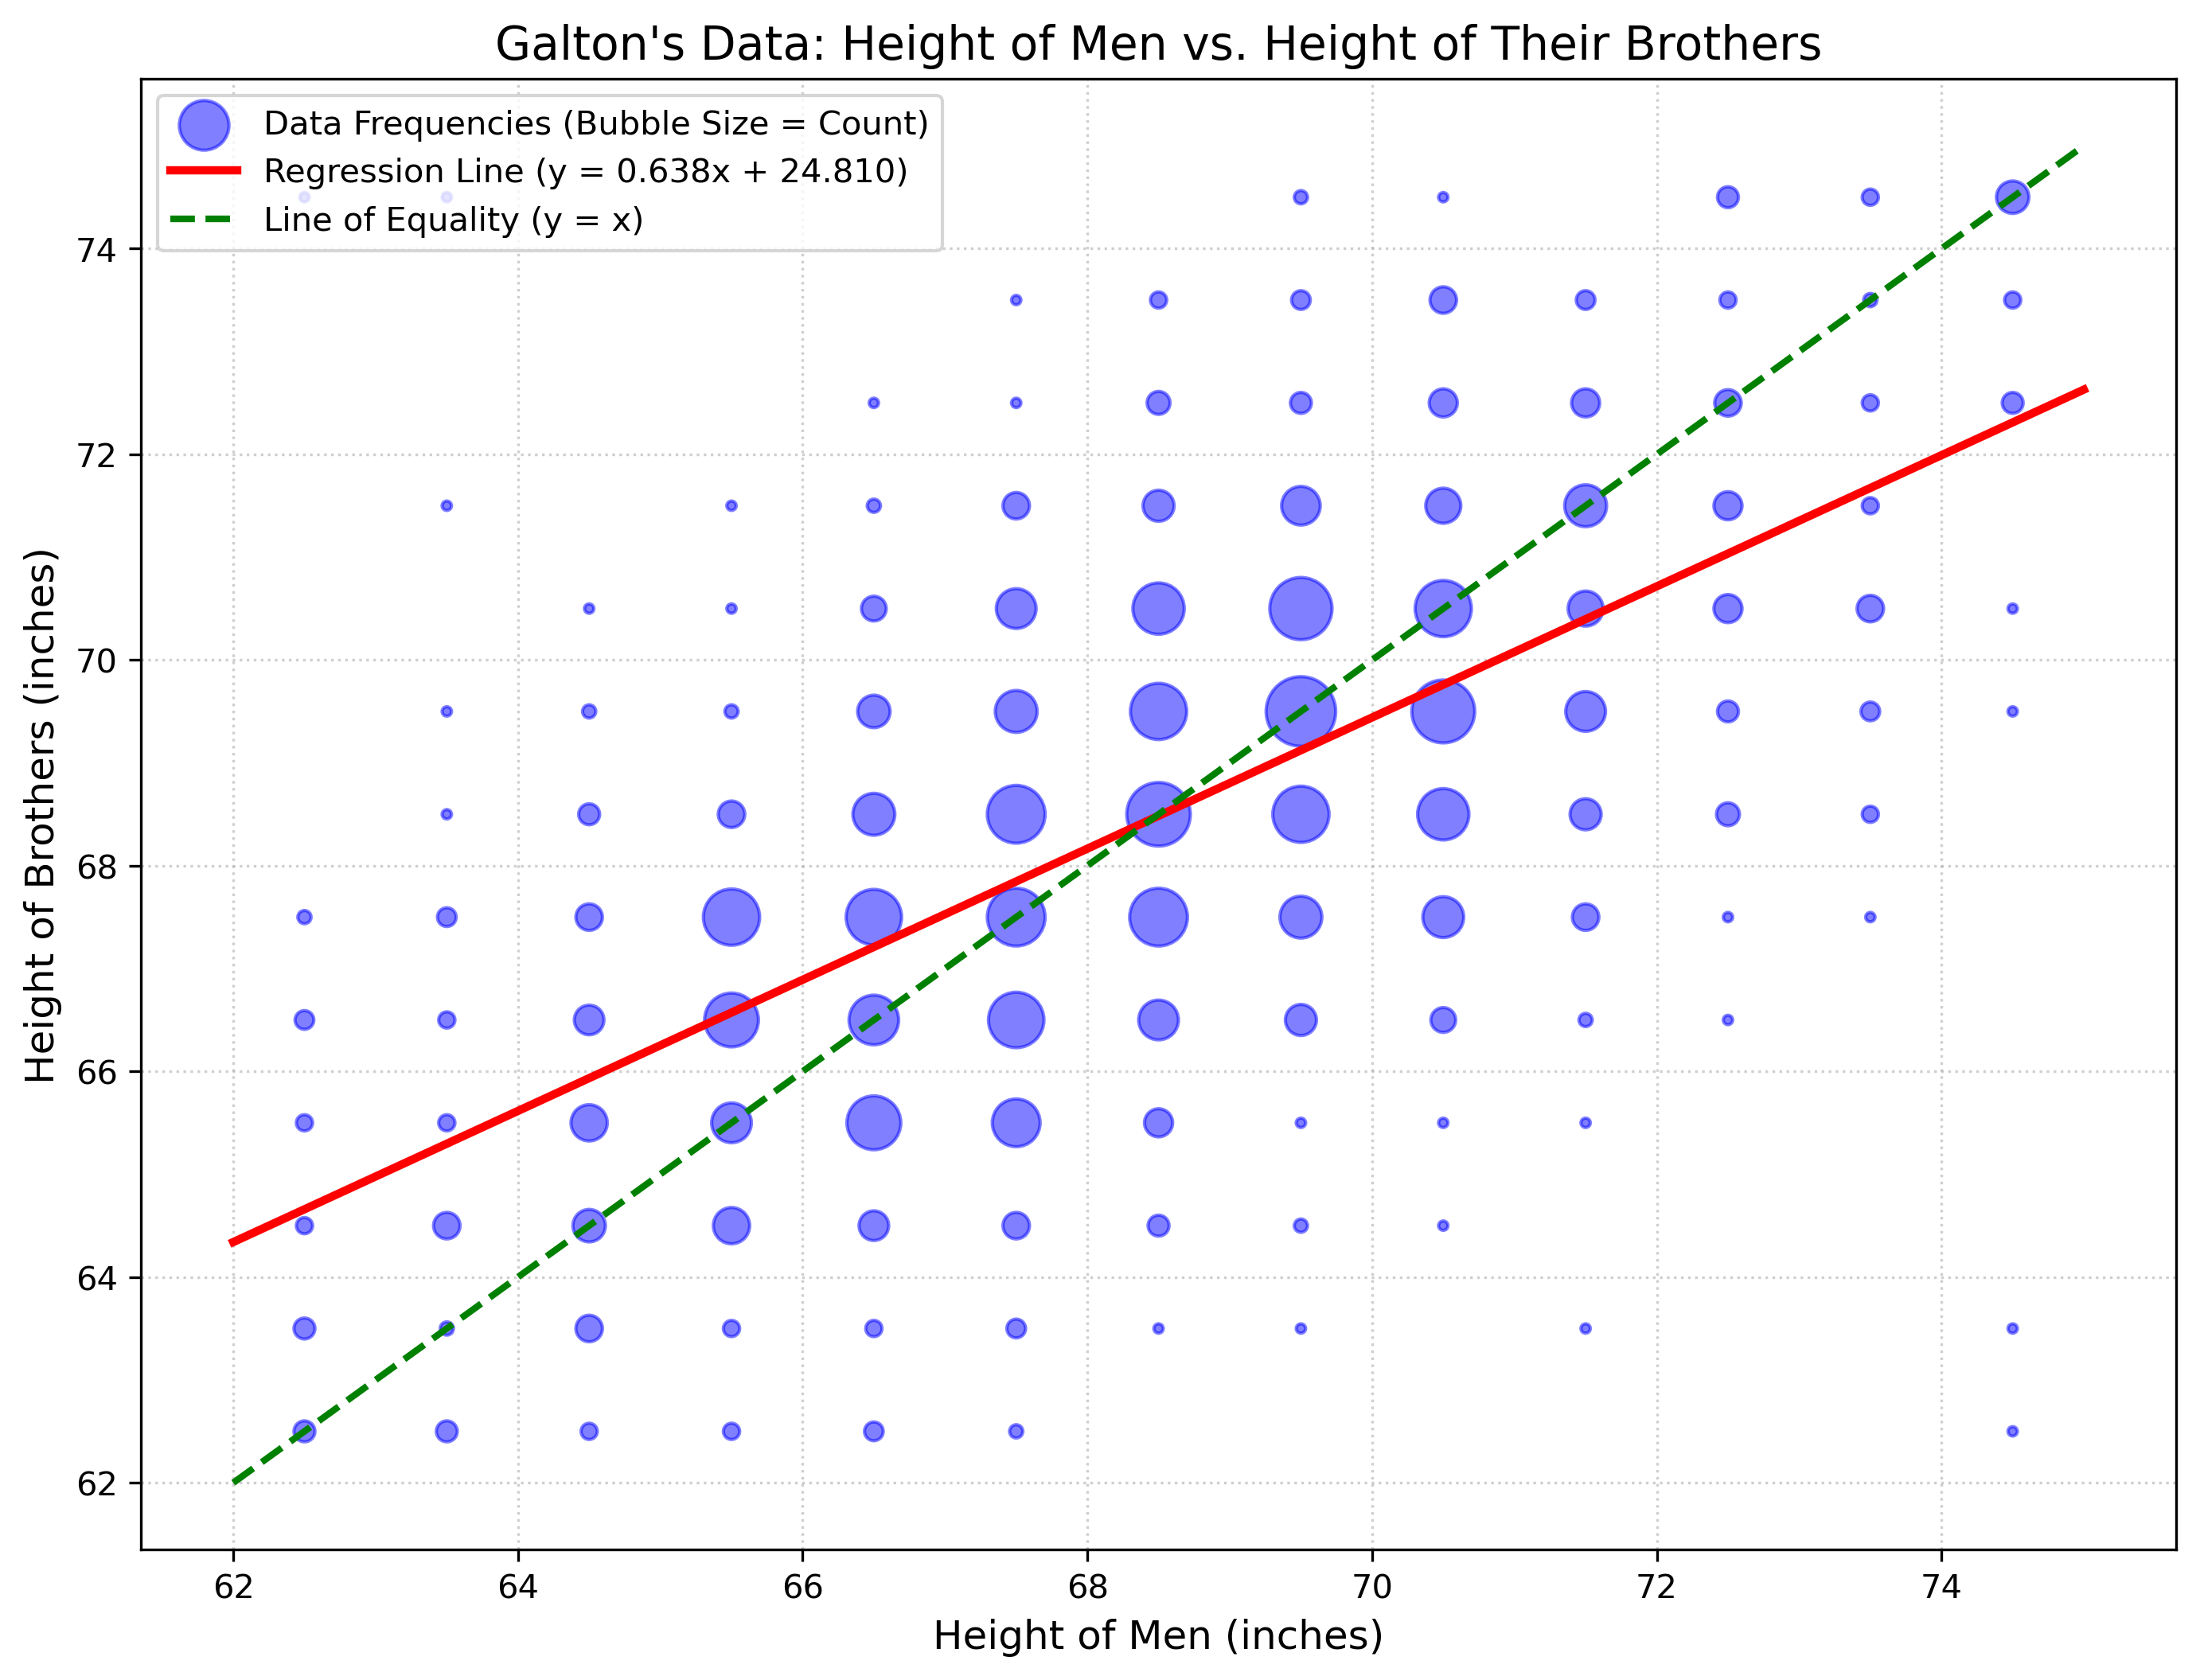
\includegraphics[width=0.8\linewidth]{galton_heights.png}\end{center}
$r = 0.63767 < 1$, showing regression to the mean, i.e. when a man is taller than average, his brother is likely to be tall, but shorter than he is.
\answer

\section*{Prob-2}
(A)
OM: Y = 0.33X
ON: X = 0.33Y

(B)
OL, OM
\answer

\section*{Prob-3}
(A)
mid-parent population: 1
each subgroup's offspring: 4, 5

(B)
经过倾斜槽仍为正态分布；
子代$S = F + V$，其中Z和V都满足正态分布且独立，根据简单计算可知S也满足正态分布；
是的吧……不然呢
\answer

\section*{Prob-4}
It's obvious the shot in a single midlevel is expected to fall directly below. Let's focus on the other part.
Assume $S = F + V$, where $F$ is the midlevel position and $V$ is the deviation from the midlevel. 

(1)Mathematically:
If $S < E(F)$, note that $E(V|S < E(F)) < 0$, which means that the expected value of V given that S is less than the expected value of F is negative.
Therefore $E(F|S < E(F)) = E(S|S < E(F)) - E(V|S < E(F)) > E(S|S < E(F))$.
The same for $S > E(F)$.

(2)Intuitively:
Exactly reverse regression to the mean.
\answer

\section*{Prob-5}
\answer
Let $X$ be the height of the randomly selected woman, and $Y$ be the height of the randomly selected man.
From the problem statement, we know:
\begin{align*}
    X &\sim \mathcal{N}(\mu_X = 65, \sigma_X^2 = 1^2 = 1) \\
    Y &\sim \mathcal{N}(\mu_Y = 68, \sigma_Y^2 = 2^2 = 4)
\end{align*}
The random variables $X$ and $Y$ are independent.

We want to find the probability that the woman is taller than the man, which is $P(X > Y)$. This is equivalent to finding $P(X - Y > 0)$.

Let $D = X - Y$. Since $X$ and $Y$ are independent and normally distributed, their difference $D$ is also normally distributed with:
\begin{align*}
    \mu_D &= \mu_X - \mu_Y = 65 - 68 = -3 \\
    \sigma_D^2 &= \sigma_X^2 + \sigma_Y^2 = 1 + 4 = 5
\end{align*}
Thus, $D \sim \mathcal{N}(-3, 5)$, and the standard deviation is $\sigma_D = \sqrt{5}$.

We standardize $D$ to find the probability:
\begin{align*}
    P(X > Y) &= P(D > 0) \\
    &= P\left( \frac{D - \mu_D}{\sigma_D} > \frac{0 - (-3)}{\sqrt{5}} \right) \\
    &= P\left( Z > \frac{3}{\sqrt{5}} \right)
\end{align*}
where $Z$ is the standard normal random variable, $Z \sim \mathcal{N}(0, 1)$.

Using standard normal tables or a calculator:
\begin{align*}
    P\left( Z > \frac{3}{\sqrt{5}} \right) &= 1 - P\left( Z \le \frac{3}{\sqrt{5}} \right) \\
    &= 1 - \Phi\left( \frac{3}{\sqrt{5}} \right) \\
    &\approx 1 - \Phi(1.3416) \\
    &\approx 1 - 0.9101 \\
    &\approx 0.0899
\end{align*}

Therefore, the probability that the woman will be taller than the man is approximately $0.0899$ or $8.99\%$.
\end{document}